Functional reactive programming allows developers to declaratively specify data dependency graphs \cite{wan2000functional}. Functional reactive programming has been applied to interactive graphics \cite{elliott1997functional} and robotics \cite{hudak2003arrows}. The Model View Controller paradigm is an approach to cleanly separate application operations into three classes. The \emph{model} contains the data structures representing the application state. The \emph{view} handles graphical presentation of the model to the user. The \emph{controller} translates user interactions (such as mouse clicks, key presses, or multi-touch gestures) into changes in the model \cite{krasner1988description}. The Model View Controller paradigm can be combined with functional reactive programming to enable straightworward creation of reactive systems based on data flow graphs.
\section{The Model Data Structure}
The Model in the Model View Controller (MVC) paradigm is responsible for:
\begin{itemize}
\item managing the state of the application,
\item allowing the Controller to change the state of the application, and 
\item notifying the view when the state of the application changes.
\end{itemize}

One simple and widely used method for structuring a Model is as a set of key-value pairs \cite{leff2001web}. This kind of model can fulfill the all of the responsibilities of a Model with three methods:

\begin{itemize}
\item $set(key, value)$ Set the value for a given key.
\item $get(key)$ Get the value for a given key.
\item $on(key, callback)$ Add a change listener for a given key. Here, $callback$ is a function that will be invoked synchronously when the value for the given key is changed.
\end{itemize}

This approach is used by popular JavaScript frameworks such as Backbone and Knockout. Using our pseudocode conventions, we will discuss one way a key-value Model can be implemented. We will first discuss a simple version with only $set$ and $get$, then discuss a more complex version that also includes $on$.
\begin{codebox}
\li $SimplestModel \gets \lambda()$ \label{simplestModelConstructor}
\Do
  \li $values = \{\,\}$ \label{simplestModelValues}
  \li \Return \label{simplestModelMethodsBegin}
  \Do
    \li $set: \lambda(key, value) \, values[key] \gets value$
    \li $get: \lambda(key)$ \Return $values[key]$ \label{simplestModelMethodsEnd}
  \End
\End
\end{codebox}

The above pseudocode implements a key-value model that has only $set$ and $get$ methods. Line \ref{simplestModelConstructor} defines the constructor function, $SimplestModel$, which will return a new object that has $set$ and $get$ methods. Line \ref{simplestModelValues} defines a private variable called $values$ that will contain the key-value mapping. Lines \ref{simplestModelMethodsBegin} - \ref{simplestModelMethodsEnd} define the $set$ and $get$ methods, which store and retreive values from the internal $values$ object. Here's an example of how $SimplestModel$ might be used.

\begin{codebox}
\li $mySimplestModel \gets SimplestModel()$
\li $mySimplestModel.set($\verb1'x'1$,5)$
\li $mySimplestModel.get($\verb1'x'1$)$ \Comment Evaluates to 5
\end{codebox}

Here is a version of the model that implements the $on$ method as well:

\begin{codebox}
\li $SimpleModel \gets \lambda()$ \label{simpleModelConstructor}
\Do
  \li $values = \{\,\}$ \label{simpleModelValues}
  \li $callbacks = \{\,\}$ \label{simpleModelCallbacks}
  \li \Return \label{simpleModelMethodsBegin}
  \Do
    \li $on: \lambda(key, callback)$ \label{simpleModelOn}
    \Do
      \li \If $callbacks[key] \isequal \const{nil}$
      \Do
        \li $callbacks[key] \gets [\,]$
      \End
      \li $callbacks[key].push(callback)$
    \End
    \li $set: \lambda(key, value)$
    \Do
      \li $values[key] \gets value$
      \li \If $callbacks[key] \neq \const{nil}$
      \Do
        \li \For $callback \in callbacks[key]$
        \Do
          \li $callback()$
        \End  
      \End
    \End
    \li $get: \lambda(key)$ \Return $values[key]$
  \End
\End
\end{codebox}

The above version includes an additional private variable, $callbacks$, which is an object whose keys are property names and whose values are arrays of callback functions. The $on$ method defined starting at line \ref{simpleModelOn} adds the given callback to the list of callbacks for the given key (and creates the list if it does not yet exist). The $set$ method has been modified to invoke the callback functions associated with the given key when the value for that key is changed. Here is an example of how the $on$ method can be used.

\begin{codebox}
\li $mySimpleModel \gets SimpleModel()$
\li $mySimpleModel.on($\verb1'x'1$, \lambda()$
\Do
  \li $log(mySimpleModel.get($\verb1'x'1$))$ \label{simpleModelCallbackPrintout}
\End
\li $)$ 
\li $mySimpleModel.set($\verb1'x'1$,5)$ \Comment Causes line \ref{simpleModelCallbackPrintout} to log 5
\li $mySimpleModel.set($\verb1'x'1$,6)$ \Comment Causes line \ref{simpleModelCallbackPrintout} to log 6
\end{codebox}

\section{Functional Reactive Change Propagation}
For complex applications such as interactive visualizations, managing propagation of changes can quickly become complex. For this reason, modular visualization environments based on data flow have become popular \cite{abram1995extended}. A data flow graph defines a directed acyclic graph of data dependencies. The data flow model is amenable to construction of visual programming languages \cite{hils1992visual}. While many systems consider data flow as a means to construct data transformation pipelines, the concept also applies to building reactive systems that manage change propagation throughout an application or subsystem in response to user interactions or other events \cite{elliott1997functional}.

To provide a solid foundation for dynamic visualization systems, the Model should be able function in the context of data dependency graphs. Developers should be able to declaratively specify data dependencies, and change propagation should be automatically managed. The $when$ operator from functional reactive programming propagates changes from one or more reactive functions (such as is found in the JavaScript libraries Bacon.js and RXJS).

Our Model implementation can be extended with a $when$ operator that enables construction of data dependency graphs. This operator will become a foundation for building dynamic interactive visualizations. Since $when$ is superior to $on$ in that it handles change propagation intelligently, in this final version $on$ is not exposed in the public Model API.

\begin{codebox}
\li $Model \gets \lambda()$
\Do
  \li $simpleModel \gets SimpleModel()$
  \li \Return
  \Do
    \li $set: simpleModel.set$
    \li $get: simpleModel.get$
    \li $when: \lambda(dependencies, fn)$
    \Do
      \li $callFn \gets debounce(\lambda()$
      \Do
        \li $args = dependencies.map(simpleModel.get)$
        \li \If $allAreDefined(args)$
        \Do
          \li $apply(fn, args)$
        \End
      \End
      \li $)$
      \li $callFn()$
      \li \For $key \in dependencies$
      \Do
        \li $simpleModel.on(key, callFn)$
      \End  
    \End
  \End
\End
\end{codebox}
\TODO{describe Model()}
\begin{codebox}
\li $debounce \gets \lambda(fn)$
\Do
  \li $queued \gets \const{false}$
  \li \Return $\lambda()$
  \Do
    \li \If $queued \isequal \const{false}$
    \Do
      \li $queued \gets \const{true}$
      \li $run(\lambda()$
      \Do
        \li $queued \gets \const{false}$
        \li $fn()$
      \End
      \li $)$
    \End
  \End
\End
\end{codebox}
\TODO{describe debounce()}
\begin{codebox}
\li $allAreDefined \gets \lambda(arr)$
\Do
  \li \For $item \in arr$
  \Do
    \li \If $item$ is undefined 
    \Do
      \li \Return $\const{false}$
    \End
  \End
  \li \Return $\const{true}$
\End
\end{codebox}
\TODO{describe allAreDefined()}

\begin{figure}[h]
  \caption{A simple data dependency graph using functional reactive models. Here, $fullName$ is recomputed whenever $firstName$ or $lastName$ change.}
  \centering
  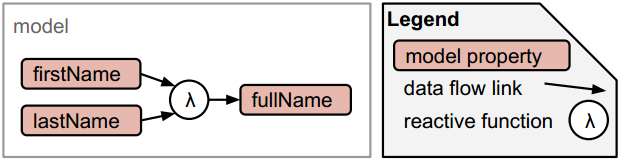
\includegraphics[width=\textwidth]{figures/computedProperty.png}
\end{figure}
\TODO{add pseudocode for each figure}
\begin{figure}[h]
  \caption{A data dependency graph with two hops. When $x$ changes, the change propagates to $y$ then to $z$.}
  \centering
  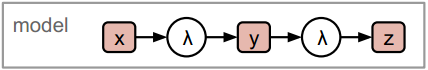
\includegraphics[width=0.7\textwidth]{figures/dependencyGraph.png}
\end{figure}

\section{Functional Reactive Visualizations}
\begin{figure}[h]
  \caption{The data dependency graph for a dynamic bar chart.}
  \centering
  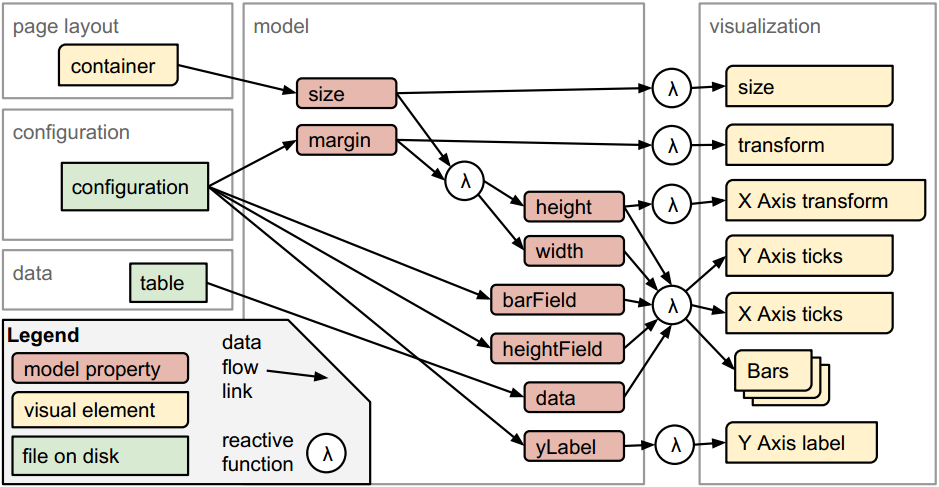
\includegraphics[width=\textwidth]{figures/barChartFlow.png}
\end{figure}
\begin{figure}[h]
  \caption{The appearance of a dynamic bar chart.}
  \centering
  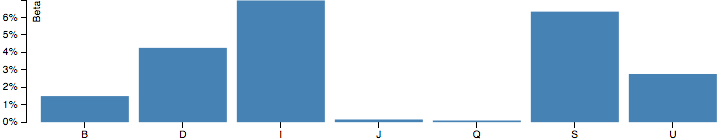
\includegraphics[width=\textwidth]{figures/barChart.png}
\end{figure}
\begin{figure}[h]
  \caption{An example of multiple linked views using functional reactive models. Brushing in the scatter plot causes the selected data to be aggregated and plotted in the bar chart. Data shown is Fisher's Iris data \cite{fisher1936use}. }
  \centering
  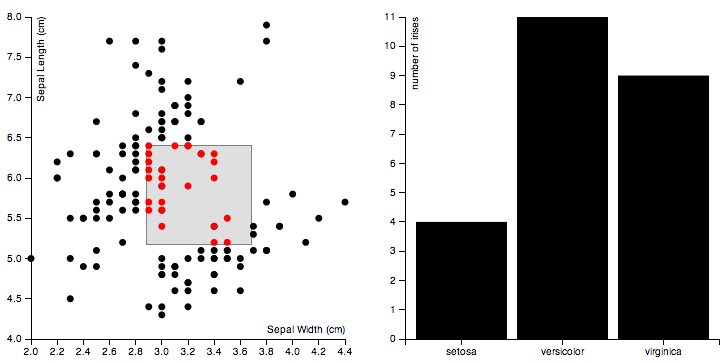
\includegraphics[width=\textwidth]{figures/linkedViews.png}
\end{figure}
